\chapter{Funciones}\label{funciones}

La función es, tal vez, uno de los conceptos más importantes en matemáticas, pues gran parte de los demás conceptos matemáticos se basan en el conocimiento de las funciones y sus propiedades. Aunque existen muchos tipos de funciones —por ejemplo, el área de un círculo que depende de su radio, el costo de un envío que depende de su peso, o la velocidad que depende del tiempo \(t\) transcurrido—, las funciones no siempre dependen de una sola variable. Por ejemplo, el volumen de un cilindro depende tanto de su altura como de su radio. 

En esta sección nos enfocaremos inicialmente en las funciones de una variable real y desarrollaremos con detalle este concepto fundamental.


\section{Propiedades básicas}

\begin{definition}[Función]
Una función \( f \) es una regla de correspondencia que asigna a cada elemento \( x \) de un conjunto denominado \textbf{dominio}, un único valor \( f(x) \) en otro conjunto, llamado \textbf{codominio}. 

El conjunto de todos los valores \( f(x) \) obtenidos se denomina \textbf{rango} o \textbf{imagen} de \( f \). Es común decir que $x$ es la variable independiente y $f(x)$ es la variable dependiente. 
\end{definition}
\begin{rem}[Formas de representar una función]
Existen básicamente cuatro formas de representar una función: verbalmente, describiendo en palabras la relación entre variables; numéricamente, mediante una tabla de valores; visualmente, a través de una gráfica; y algebraicamente, por medio de una fórmula explícita. Aclararemos estas formas en el siguiente ejemplo.
\end{rem}

\begin{example}\label{funcioncosto}
Un contenedor rectangular sin tapa tiene un volumen de \(10\,\text{m}^3\). La longitud de su base es dos veces su ancho. El material para la base cuesta \$10 por metro cuadrado y el material para los lados cuesta \$6 por metro cuadrado. Exprese el costo de los materiales como una función del ancho de la base. Dé una representación verbal, numérica, visual y algebraica.

\begin{myproof}
Primero introducimos las variables geométricas del problema. Sea \(x\) el ancho de la base (en metros), \(2x\) la longitud de la base (en metros) y \(h\) la altura del contenedor (en metros). Como el contenedor no tiene tapa, solo hay base y cuatro lados.

La condición de volumen se escribe como
\[
V = (\text{ancho})\cdot(\text{longitud})\cdot(\text{altura}) = x \cdot 2x \cdot h = 2x^{2}h = 10.
\]
Despejamos la altura en función del ancho:
\[
h = \frac{10}{2x^{2}} = \frac{5}{x^{2}}.
\]

Ahora calculamos el área de cada parte para expresar el costo total. 
El área de la base es
\[
A_{\text{base}} = x \cdot 2x = 2x^{2},
\]
y su costo es
\[
C_{\text{base}} = 10 \cdot A_{\text{base}} = 10 \cdot 2x^{2} = 20x^{2}.
\]

El contenedor tiene cuatro lados rectangulares: dos lados de dimensiones \(x \times h\) y dos de dimensiones \(2x \times h\). El área total de los lados es
\[
A_{\text{lados}} = 2(xh) + 2(2xh) = 2xh + 4xh = 6xh.
\]
Sustituimos \(h = \dfrac{5}{x^{2}}\):
\[
A_{\text{lados}} = 6x \cdot \frac{5}{x^{2}} = \frac{30}{x}.
\]
El costo de los lados es entonces
\[
C_{\text{lados}} = 6 \cdot A_{\text{lados}} = 6 \cdot \frac{30}{x} = \frac{180}{x}.
\]

Sumando ambos aportes obtenemos el costo total como función del ancho \(x\):
\[
C(x) = C_{\text{base}} + C_{\text{lados}} = 20x^{2} + \frac{180}{x}.
\]

Podemos ahora presentar las cuatro representaciones de la función costo:

\textbf{Representación verbal:} A cada valor positivo del ancho \(x\) se le asigna el costo total de construir el contenedor, sumando el costo de la base y el de los cuatro lados, donde la longitud es \(2x\) y la altura se ajusta para que el volumen sea \(10\,\text{m}^3\).

\textbf{Representación algebraica:} La función costo en términos del ancho \(x\) está dada por
\[
C(x) = 20x^{2} + \frac{180}{x}, \quad x > 0.
\]

\textbf{Representación numérica:} Podemos elaborar una tabla de valores, eligiendo algunos anchos \(x\) (en metros) y calculando el costo \(C(x)\) (en dólares). Por ejemplo:
\[
\begin{array}{c|c}
x & C(x) \\
\hline
1   & 20(1)^{2} + \dfrac{180}{1}   = 200 \\
1.5 & 20(1.5)^{2} + \dfrac{180}{1.5} = 20\cdot 2.25 + 120 = 165 \\
2   & 20(2)^{2} + \dfrac{180}{2}   = 80 + 90 = 170 \\
2.5 & 20(2.5)^{2} + \dfrac{180}{2.5} = 20\cdot 6.25 + 72 = 197 \\
\end{array}
\]

\textbf{Representación visual:} La representación gráfica consiste en dibujar la curva de la función
\[
y = C(x) = 20x^{2} + \frac{180}{x}, \quad x > 0,
\]
en el plano \(xy\), donde el eje horizontal representa el ancho \(x\) y el eje vertical representa el costo \(C(x)\). Esta gráfica muestra cómo varía el costo total según el ancho de la base.
\begin{figure}[H]
\centering
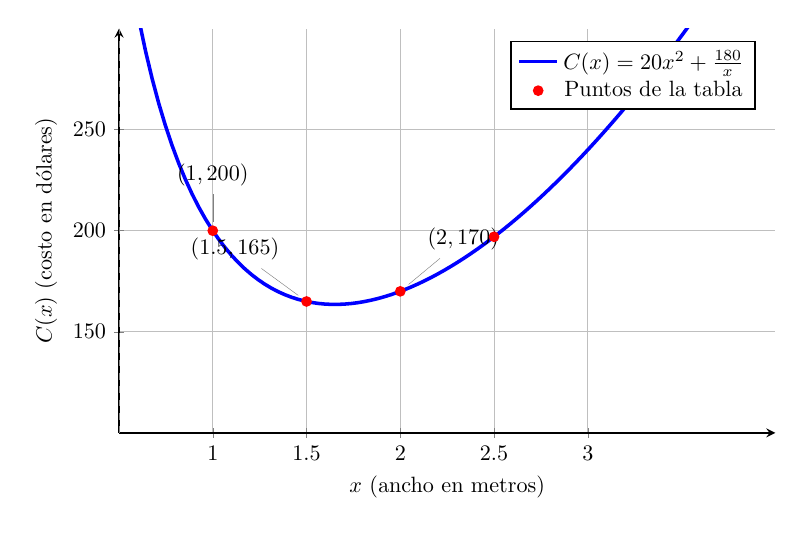
\begin{tikzpicture}[scale=0.8]
% Definir la función
\begin{axis}[
    width=12cm,
    height=8cm,
    xlabel={$x$ (ancho en metros)},
    ylabel={$C(x)$ (costo en dólares)},
    xmin=0.5, xmax=4,
    ymin=100, ymax=300,
    grid=major,
    axis lines=left,
    xtick={1,1.5,2,2.5,3},
    ytick={150,200,250},
    legend pos=north east,
    domain=0.5:4,
    samples=100,
    thick
]

% Graficar la función C(x)
\addplot[blue, ultra thick] {20*x^2 + 180/x};
\addlegendentry{$C(x)=20x^2+\frac{180}{x}$}

% Marcar los puntos de la tabla numérica
\addplot[red, mark=*, only marks] coordinates {
    (1,200)
    (1.5,165)
    (2,170)
    (2.5,197)
};
\addlegendentry{Puntos de la tabla}

% Etiquetas de los puntos clave
\node[pin=90:{$(1,200)$}] at (axis cs:1,200) {};
\node[pin=120:{$(1.5,165)$}] at (axis cs:1.5,165) {};
\node[pin=60:{$(2,170)$}] at (axis cs:2,170) {};

% Línea vertical en x=0 (asíntota)
\draw[dashed, gray] (axis cs:0.5,100) -- (axis cs:0.5,300) node[above right] {asíntota};

\end{axis}
\end{tikzpicture}
\caption{Figura del ejemplo \ref{funcioncosto}}

\end{figure}
Con esto hemos descrito el costo como función del ancho en sus cuatro formas: verbal, numérica, visual y algebraica.
\end{myproof}
\end{example}



\begin{prob} 
Demuestre que $z$ es imaginario puro si y solo si $z=-\overline{z}$.
\begin{myproof}
Sea $z \in \mathbb{C}$. Recordemos que $z$ es imaginario puro si y solo si su parte real es cero, es decir, $z = bi$ con $b \in \mathbb{R}$.

\textbf{($\Rightarrow$)} Supongamos que $z$ es imaginario puro.  
Entonces $z = bi$ con $b \in \mathbb{R}$.  
El conjugado es $\overline{z} = \overline{bi} = -bi$.  
Por lo tanto,
\[
-\overline{z} = -(-bi) = bi = z.
\]
Así, $z = -\overline{z}$.

\textbf{($\Leftarrow$)} Supongamos que $z = -\overline{z}$.  
Sea $z = a + bi$ con $a, b \in \mathbb{R}$.  
Entonces $\overline{z} = a - bi$ y la igualdad se convierte en:
\[
a + bi = - (a - bi) = -a + bi
\]
Comparando partes reales:
\[
a = -a \implies a = 0
\]
Por lo tanto, $z = 0 + bi = bi$, es decir, $z$ es imaginario puro.

\textbf{Conclusión:}  
$z$ es imaginario puro si y solo si $z = -\overline{z}$.
\end{myproof}

\end{prob}